\input sys/inputs.tex

\begin{document}

\bigheading{Connect Highways}

% \info{task_name}{infile}{outfile}{points}{timelimit}{memlimit}
% leave this values, if you are not interested
\info{networks}{stdin}{stdout}{100}{400 ms}{32 MiB}

In Byteland, there are two highway networks operated by two companies: Red and Blue. Both networks consist of junction points and straight lines connecting pairs of junction points, called segments. Any two segments are non-crossing, meaning that they can only touch at junction points. Both networks are connected, that is any two junction points are connected through a series of consecutive segments. Moreover, the two systems are disjoint, i.e., no junction point appears in both networks.
The two companies have now decided to fuse into a single one, and they want to connect their networks by building a straight line segment between two junction points, one in each network. The new segment cannot cross any existing segment.

\heading{Task}
Write a program that computes a suitable connecting segment.

\heading{Input}
The input contains the description of the Red, followed by the description of the Blue network. The first line of the description contains two integers $N$ ($2 \leq N \leq 200000$) and $M$ ($1 \leq M \leq 700000$). $N$ is the number of the junction points and $M$ is the number of the segments. Each of the following $N$ lines contains two integers $x$ and $y$ ($-1000000 \leq x,y \leq 1000000$), which are the coordinates of a junction point. Each of the following $M$ lines contains two integers $p$ and $q$ ($1\leq p \neq q \leq N$), the endpoints of a segment. Junction points are identified by the numbers $1,\ldots,N$ in the order of their appearance in the input.

\bigskip
In the $30\%$ of the testcases the number of the junction point and the number of the segments are not larger than $3 000$ in both networks.

\heading{Output}
The first and only line of the output contains two integers u and v, the endpoints of a connecting segment. That is, $u$ is junction point of the Red, $v$ is a junction point of the Blue network and the line segment with endpoints $u$ and $v$ crosses no segment of any of the networks. If there are multiple solutions, your program should output only one; it does not matter which one.

\heading{Samples}

\sampleIN
5 6
0 3
1 1
6 0
5 3
9 8
1 2
1 3
4 3
3 5
1 5
2 3
4 4
6 4
4 4
4 2
2 3
1 2
4 2
2 3
3 4
\sampleOUT
5 1
\sampleCOMMENT
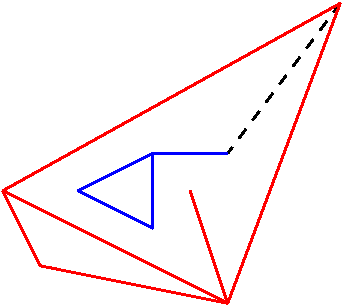
\includegraphics[height=4cm]{img/fig11.pdf}
\sampleEND

\end{document}
